\chapter{Technical Performance}\label{ch:testing}
% Generated data test outcomes.
% how good the training is and how good the system is before putting a human in the loop.
Before testing the system on human subjects, we performed a series of tests to evaluate the performance of the system on generated data. 
The tests were designed to evaluate the performance of the system in terms of the following:
The chapter is divided into four sections, we will discuss the classification accuracy, which is the capabilty of the system to correctly classify the input data, the latency, wich is the classification speed of the system, and the robustness of the system, which represents the tolerance to noise and errors in the input data, along with other performance metrics, such as efficiency and portability that we could not deeply verify in this stage of the project.
The results of the tests indicate that the system is able to classify the generated data with high accuracy, in competitive time, and with low resource usage.
The system is able to handle errors and noise in the data, and should be able to run on most modern hardware platforms.
We will discuss the results of the human study in the next chapter (Chapter~\ref{ch:human_study}).

\section{Classification Accuracy}
% How good the system is at classifying the data.
The classification accuracy is a measure of how well the system is able to correctly classify the data.
The classification accuracy is calculated as the percentage of correctly classified data points over the total number of data points.
The classification accuracy is an important metric for evaluating the performance of the system, as it provides an indication of how well the system is able to distinguish between different classes of data.
During the training we computed the training and validation accuracy of the system, the first metric on the train dataset, to verify wether the network was actually learning, and the second metric on a part of the dataset that was not used for training.
During the tests, we evaluated the classification accuracy of the system on generated data.
We will compare these results with the classification accuracy of the system on human subjects in the next chapter.

\subsection*{Train and Validation Accuracy}
The train accuracy is the percentage of correctly classified data points over the total number of data points in the train dataset.
During our training, the train accuracy of the system was 71.37\%.
This result indicates that the system is able to correctly classify the training data.

The validation accuracy is the percentage of correctly classified data points over the total number of data points in the validation dataset.
During our training, the validation accuracy of the system was 47.23\%.
This score is significantly lower than the train accuracy, which indicates that the system is overfitting the training data.
This means that the system is not able to generalize well to new data.
This is a common problem in machine learning, and can be addressed by using techniques such as regularization, dropout, and data augmentation.

\begin{table}[!htbp]
    \centering
    \begin{tabular}{|c||c|c|c|c|}
        \hline
        & \textbf{Feet} & \textbf{Left Hand} & \textbf{Right Hand} & \textbf{Rest} \\
        \hline
        \hline
        \textbf{Feet} & \textbf{779} & 367 & 259 & 314 \\
        \hline
        \textbf{Left Hand} & 284 & \textbf{1005} & 189 & 258 \\
        \hline
        \textbf{Right Hand} & 356 & 243 & \textbf{840} & 268 \\
        \hline
        \textbf{Rest} & 1474 & 1188 & 1158 & \textbf{3067} \\
        \hline
    \end{tabular}
    \caption{Confusion matrix of the validation dataset.}\label{tab:confusion_matrix}
\end{table}

Apart from the accuracy metric, we also computed the confusion matrix of the validation dataset, which is shown in Table~\ref{tab:confusion_matrix}.
In this table, it is possible to see the number of data points that were classified as each class.
The diagonal of the matrix represents the number of correctly classified data points, while the off-diagonal elements represent the number of incorrectly classified data points.
From the confusion matrix, it is possible to see that the system is able to correctly classify most of the data points for each class, therefore, altrough the validation accuracy is low, in our opinion, in a real case scenario, the system would be able to correctly classify most of the data points and therefore be useful to the end user in controlling external devices.

\subsection*{Generated Data Accuracy}
Differently from the validation dataset, the classification accuracy of the system on the generated data was 89.15\%.
This result indicates that the system is able to correctly classify the artificial data.
The confusion matrix of the generated data is shown in Table~\ref{tab:gan_confusion_matrix}.
From the confusion matrix, it is possible to see that the system is able to correctly classify most of the data points for each class, and that the system is able to distinguish between different classes of data.
\begin{table}[!htbp]
    \centering
    \begin{tabular}{|c||c|c|c|c|}
        \hline
        & \textbf{Feet} & \textbf{Left Hand} & \textbf{Right Hand} & \textbf{Rest} \\
        \hline
        \hline
        \textbf{Feet} & \textbf{824} & 104 & 38 & 34 \\
        \hline
        \textbf{Left Hand} & 16 & \textbf{961} & 1 & 22 \\
        \hline
        \textbf{Right Hand} & 28 & 51 & \textbf{789} & 132 \\
        \hline
        \textbf{Rest} & 1 & 6 & 1 & \textbf{992} \\
        \hline
    \end{tabular}
    \caption{Confusion matrix of the GAN generated data.}\label{tab:gan_confusion_matrix}
\end{table}


\section{Latency}
% How fast the system is at classifying the data.
The latency is a measure of how fast the system is able to classify the data.
The latency is calculated as the time taken by the system to classify a data point.
The latency is an important metric for evaluating the performance of the system, as it provides an indication of how fast the system is able to respond to new data and to the user input.
Since the classification time does not depend on the type of datapoint received, we tested the latency of the system on dataset data.
The average latency of the system was 5.70 millseconds, with the minimum latency being 1.10 milliseconds and the maximum latency being 24.67 milliseconds.

It is important to note that the system used 500 milliseconds EEG recordings, and, as discussed in~\cite{trafton2014blink} the average human brain image processing time is between 13 and 80 milliseconds, after that, it will take between 100 and 140 milliseconds to elaborate a motor response.
Therefore we estimate that, the system will require between 600 and 750 milliseconds to process the data and provide a response, which is fairly close to the 500 milliseconds of the EEG recording and in our opinion is an acceptable delay for EEG controlled real-time applications and devices.
Figure~\ref{fig:latency} summarizes the latency results in a real case scenario.
The figure only shows the latency of the system, and does not include the time required to communicate the classification outcome to the device and the time required by the device to respond to the classification outcome.
\begin{figure}[!htbp]
    \scalebox{1.2}[1.2]{
    \begin{tikzpicture}
        % Horizontal line
        \draw[thick] (0,0) -- (7.6625,0);
        \draw[thick, dashed] (7.6625,0) -- (8.15,0);
        \draw[thick, -Triangle] (8.15,0) -- (10,0) node[font=\scriptsize,below left=3pt and -8pt]{\textbf{ms}};
        % \draw[thick, dashed] (9,0) -- (9.5,0);
        % \draw[thick, -Triangle] (9,0) -- (10,0) node[font=\scriptsize,below left=3pt and -8pt]{\textbf{ms}};

        % Start of the timeline
        \draw (0,-0.1) -- (0,0.1) node[font=\scriptsize,below left=3pt and -6pt]{\textbf{0}};
        \node[font=\scriptsize,left=3pt] at (0,0) [anchor=east]{\textbf{Min}};

        % Image Processing Time
        \draw (0.1625, -0.1) -- (0.1625, 0.1) node[font=\scriptsize,below left=3pt and -10pt]{\textbf{\textcolor{olive}{13}}};
        \fill[purple] (0, 0.2) rectangle (0.1625, 0.4);
        
        % \draw (1, -0.1) -- (1, 0.1) node[font=\scriptsize,below left=3pt and -8pt]{\textbf{\textcolor{red}{80}}};
        % \fill[purple] (0,-0.4) rectangle (1,-0.6);
        
        % Motor Response Time
        \draw (1.4125, -0.1) -- (1.4125, 0.1) node[font=\scriptsize,below left=3pt and -10pt]{\textbf{\textcolor{olive}{113}}};
        \fill[blue] (0.1625, 0.4) rectangle (1.4125, 0.6);

        % \draw (2.75, -0.1) -- (2.75, 0.1) node[font=\scriptsize,below left=3pt and -10pt]{\textbf{\textcolor{red}{220}}};
        % \fill[blue] (1,-0.6) rectangle (2.75,-0.8);

        % Motor Response Recording Time
        \draw (7.6625, -0.1) -- (7.6625, 0.1) node[font=\scriptsize,below left=3pt and -8pt]{\textbf{\textcolor{olive}{613}}};
        \fill[red] (1.4125, 0.6) rectangle (7.6625, 0.8);

        % \draw (9, -0.1) -- (9, 0.1) node[font=\scriptsize,below left=3pt and -10pt]{\textbf{\textcolor{red}{720}}};
        % \fill[red] (2.75,-0.8) rectangle (9,-1);

        % Signal Classification Time
        \draw (8.15, -0.1) -- (8.15, 0.1) node[font=\scriptsize,below left=3pt and -10pt]{\textbf{\textcolor{olive}{615}}};
        \fill[amethyst] (7.6625, 0.8) rectangle (8.15, 1);

        % \draw (9.5, -0.1) -- (9.5, 0.1) node[font=\scriptsize,below left=3pt and -10pt]{\textbf{\textcolor{red}{732}}};
        % \fill[amethyst] (9,-1) rectangle (9.5,-1.2);

        % diff curly brace
        % \draw [decorate,decoration={brace,amplitude=5pt}] (8.15, 1) -- (9.5,1) node [anchor=south,midway,above=4pt] {\footnotesize Signal Received by Application};
    \end{tikzpicture}
    }
    \scalebox{1.2}[1.2]{
    \begin{tikzpicture}
            % Horizontal line
            \draw[thick] (0,0) -- (9,0);
            % \draw[thick, dashed] (7.6625,0) -- (8.15,0);
            % \draw[thick] (8.15,0) -- (9,0);
            \draw[thick, dashed] (9,0) -- (9.5,0);
            \draw[thick, -Triangle] (9.5,0) -- (10,0) node[font=\scriptsize,below left=3pt and -8pt]{\textbf{ms}};

            % Start of the timeline
            \draw (0,-0.1) -- (0,0.1) node[font=\scriptsize,below left=3pt and -6pt]{\textbf{0}};
            \node[font=\scriptsize,left=3pt] at (0,0) [anchor=east]{\textbf{Max}};

            % Image Processing Time
            % \draw (0.1625, -0.1) -- (0.1625, 0.1) node[font=\scriptsize,below left=3pt and -10pt]{\textbf{\textcolor{olive}{13}}};
            % \fill[purple] (0, 0.2) rectangle (0.1625, 0.4);
            
            \draw (1, -0.1) -- (1, 0.1) node[font=\scriptsize,below left=3pt and -8pt]{\textbf{\textcolor{red}{80}}};
            \fill[purple] (0,0.2) rectangle (1,0.4);
            
            % Motor Response Time
            % \draw (1.4125, -0.1) -- (1.4125, 0.1) node[font=\scriptsize,below left=3pt and -10pt]{\textbf{\textcolor{olive}{113}}};
            % \fill[blue] (0.1625, 0.4) rectangle (1.4125, 0.6);

            \draw (2.75, -0.1) -- (2.75, 0.1) node[font=\scriptsize,below left=3pt and -10pt]{\textbf{\textcolor{red}{220}}};
            \fill[blue] (1,0.4) rectangle (2.75,0.6);

            % Motor Response Recording Time
            % \draw (7.6625, -0.1) -- (7.6625, 0.1) node[font=\scriptsize,below left=3pt and -8pt]{\textbf{\textcolor{olive}{613}}};
            % \fill[red] (1.4125, 0.6) rectangle (7.6625, 0.8);

            \draw (9, -0.1) -- (9, 0.1) node[font=\scriptsize,below left=3pt and -10pt]{\textbf{\textcolor{red}{720}}};
            \fill[red] (2.75,0.6) rectangle (9,0.8);

            % Signal Classification Time
            % \draw (8.15, -0.1) -- (8.15, 0.1) node[font=\scriptsize,below left=3pt and -10pt]{\textbf{\textcolor{olive}{614}}};
            % \fill[amethyst] (7.6625, 0.8) rectangle (8.15, 1);

            \draw (9.5, -0.1) -- (9.5, 0.1) node[font=\scriptsize,below left=3pt and -10pt]{\textbf{\textcolor{red}{745}}};
            \fill[amethyst] (9,0.8) rectangle (9.5,1);

            % diff curly brace
            % \draw [decorate,decoration={brace,amplitude=5pt}] (8.15, 1) -- (9.5,1) node [anchor=south,midway,above=4pt] {\footnotesize Signal Received by Application};    
    \end{tikzpicture}
    }
    \begin{itemize}
        \item \textcolor{purple}{Brain Processing Image Time:} 13-80 ms
        \item \textcolor{blue}{Brain Motor Response Activation Time:} 100-140 ms
        \item \textcolor{red}{BCI Motor Response Recording Time:} 500 ms
        \item \textcolor{amethyst}{Signal Classification Time:} 1.10-24.67 ms
    \end{itemize}
    \caption{Latency of the system in a real case scenario.}\label{fig:latency}
\end{figure}

\section{Robustness}
% How well the system performs in case of errors or noise in the data.
The robustness is a measure of how well the system performs in case of errors or noise in the data.
The robustness is an important metric for evaluating the performance of the system, as it provides an indication of how well the system is able to handle errors and noise in the data.
During the tests, we evaluated the robustness of the system by testing the classificator on data with different levels of Gaussian noise on dataset and GAN generated data.
Since the accuracy, as seen in the previous section, is not an extremely accurate metric, we computed the confusion matrix of the system on the noisy data.
We run tests with increasing levels of Gaussian noise, with a standard deviation going from 0.0 to 9.9 in steps of 0.1 and a mean of 0.0 and e noticed that the system is able to correctly classify most of the data points for each class, in all the cases.
While in depth results are shown in Appendix~\ref{app:robustness}, in Figure~\ref{fig:robustness} we show the precision of the system on the noisy data.
As it is visible, the precision on GAN generated data is higher than the one on the dataset data, and the precision decreases as the noise level increases, but the system is still able to correctly classify most of the data points for each class, even in the presence of high level of noise.
\begin{figure}[!htbp]
    \centering
    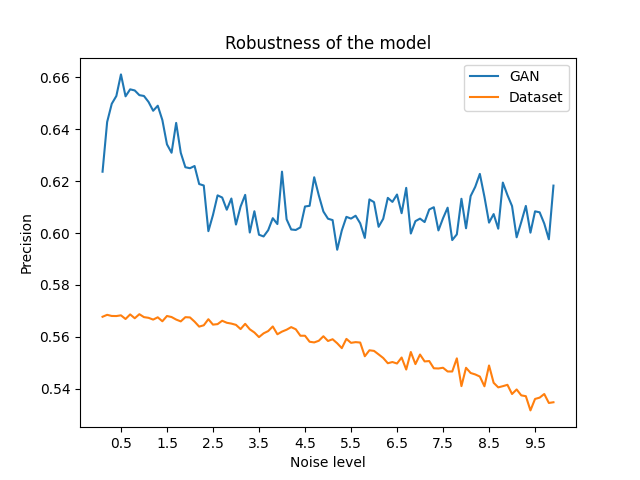
\includegraphics[width=0.8\textwidth]{Figures/Testing/robustness_plot}
    \caption{Robustness of the system in case of noise in the data.}\label{fig:robustness}
\end{figure}

\section{Other Performance Metrics}
In this section, we will discuss a set of other performance metrics that we consider important, but that we could not deeply verify in this stage of the project.
These metrics include portability, which is a measure of how well the system performs on different platforms, efficiency, which is a measure of how well the system performs in terms of resource usage, and maintainability, which is a measure of how well the system performs in terms of code quality and documentation.

\paragraph{Portability}
% How well the system performs on different platforms.
The portability is a measure of how well the system performs on different platforms.
The portability is an important metric for evaluating the performance of the system, as it provides an indication of how well the system is able to run on different hardware and software platforms.
During the tests, we could not evaluate the portability due to the lack of different hardware and software platforms.
However, we believe that the system should be able to run on different platforms, as it is written in Python 3.10 and based on standard machine learning libraries and does not require any specialized hardware or software, except for the EEG device and the CUDA-enabled GPU.
As we will discuss in the next paragraph, we evaluated the hardware requirements of the system, and we believe that the system should be able to run flawlessly on most modern hardware platforms.

\paragraph{Efficiency}
% How well the system performs in terms of resource usage.
The efficiency is a measure of how well the system performs in terms of resource usage.
The efficiency is an important metric for evaluating the performance of the system, as it provides an indication of how well the system is able to use the available resources.
During the tests, we evaluated the efficiency of the system by measuring the Floating Point Operations per Second (FLOPS), CPU memory and GPU (CUDA) memory usage of the system during the classification of the data.

\begin{table}[!htbp]
    \centering
    \begin{tabular}{|c||c|c|c|}
        \hline
        \textbf{Resource} & \textbf{Minimum Usage} & \textbf{Average Usage} & \textbf{Maximum Usage} \\
        \hline
        \hline
        FLOPS & 754400 & 754400 & 754400\\
        \hline
        CPU Memory & 30176 B & 47000 B & 90512 B \\
        \hline
        GPU CUDA Memory & 277504 B & 17765330 B  & 41378304 B \\
        \hline
    \end{tabular}
    \caption{Efficiency of the system in terms of resource usage.}\label{tab:efficiency}
\end{table}
The results summary of the tests are shown in Table~\ref{tab:efficiency}.
As it is visible, the system requires a low amount of resources, $\le$~755~K-FLOPS, $\approx$~47~KB RAM and $\approx$~18~MB VRAM, and should be able to run on most modern hardware platforms.
Detailed results are shown in Appendix~\ref{app:resource_usage}.

\paragraph{Maintainability}
% How well the system performs in terms of code quality and documentation.
The maintainability is a measure of how well the system performs in terms of code quality and documentation.
The maintainability is an important metric for evaluating the performance of the system, as it provides an indication of how well the system is able to be maintained and extended.
During the tests, we evaluated the maintainability of the system by measuring the code quality and documentation of the system.
The code quality of the system was evaluated using the Pylint tool, which is a static code analysis tool for Python.
The Pylint tool provides a score between 0 and 10, where 0 is the worst score and 10 is the best score.
The code quality of the system was 6.55, which indicates that the system has a moderate code quality, and that there is room for improvement.
Unfortunately, as of now, the system does not have any documentation, and we believe that the system should be documented to make it easier to maintain and extend.

\section{Performance Discussion}
% Summary of the testing results.
In summary, before testing the system on human subjects, we performed a series of tests to evaluate the performance of the system on realistic data.
The tests were designed to evaluate the performance of the system in terms of classification accuracy, latency and robustness, as well as other important performance indicators like portability, efficiency and maintainability.
The results of the tests indicate that the system is able to classify the generated data with high accuracy.
The classification is performed in competitive time, allowing for real-time applications with an acceptable delay and error.
The system is able to handle errors and noise in the data, and should be able to run on most modern hardware platforms, with low resource usage.
Of course, as of now, the system has only been tested on generated data, and further testing is required to evaluate the performance of the system on human subjects.
We will discuss the results of the human study in the next chapter.
